% use "latex" to generate a *.dvi file, and use "dvisvgm --no-fonts" to convert to .svg
\documentclass[border=10pt]{standalone}
\usepackage{tikz}

\begin{document}

\centering

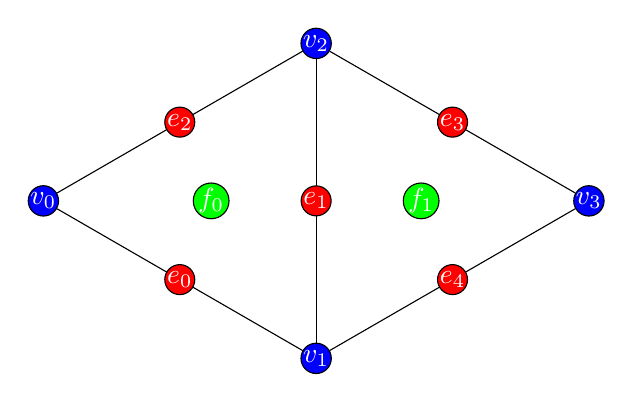
\begin{tikzpicture}[scale=2.0]
  \tikzstyle{vertex}  = [text=blue]
  \tikzstyle{vertexV} = [circle,inner sep=0pt,draw=black,fill=blue,text=white]
  \tikzstyle{edge}    = [text=red]
  \tikzstyle{edgeV}   = [circle,inner sep=0pt,draw=black,fill=red,text=white]
  \tikzstyle{face}    = [text=green]
  \tikzstyle{faceV}   = [circle,inner sep=0pt,draw=black,fill=green,text=white]
  \tikzstyle{sec}     = [->]
  % Doublet mesh with values for P_3
  \path (-1.732, 0.0) node[vertexV](dv0) {$v_0$};
  \path ( 0.0,  -1.0) node[vertexV](dv1) {$v_1$};
  \path ( 0.0,   1.0) node[vertexV](dv2) {$v_2$};
  \path ( 1.732, 0.0) node[vertexV](dv3) {$v_3$};
  \draw (dv0) -- (dv1) node[edgeV,pos=0.5] {$e_0$};
  \draw (dv1) -- (dv2) node[edgeV,pos=0.5] {$e_1$};
  \draw (dv2) -- (dv0) node[edgeV,pos=0.5] {$e_2$};
  \draw (dv2) -- (dv3) node[edgeV,pos=0.5] {$e_3$};
  \draw (dv3) -- (dv1) node[edgeV,pos=0.5] {$e_4$};
  \path (-0.6667, 0.0) node[faceV](f0) {$f_0$};
  \path ( 0.6667, 0.0) node[faceV](f1) {$f_1$};
\end{tikzpicture}

\end{document}
